% Shared preamble for the Week 7 student pages (Take-away games)
\documentclass[12pt]{article}
\usepackage[letterpaper, top=0.85in, bottom=0.8in, left=0.75in, right=0.75in,
            headheight=18pt, headsep=16pt, footskip=30pt]{geometry}
\usepackage{fontspec}
\setmainfont{Andika}
\usepackage{fancyhdr}
\usepackage{tikz}
\usetikzlibrary{shapes.geometric, calc}
\usepackage{array}

\pagestyle{fancy}
\fancyhf{}
\renewcommand{\headrulewidth}{0.5pt}
\renewcommand{\footrulewidth}{0pt}
\fancyfoot[L]{\fontsize{11}{13}\selectfont Bellingham Math Circle / Week 7}
\fancyfoot[R]{\fontsize{11}{13}\selectfont \thepage}
\newcommand{\header}[1]{\fancyhead[L]{\fontsize{12}{14}\selectfont\bfseries Week 7 / Take-away games / #1}}

\setlength{\parindent}{0pt}
\setlength{\parskip}{0pt}
\newcommand{\problem}[1]{\par\textbf{Problem #1:}~}
\hyphenpenalty=10000
\exhyphenpenalty=10000
\AtBeginDocument{\raggedright}

% ---------- drawing styles ----------
\tikzset{
  ctr/.style={circle, draw=black, line width=0.9pt, fill=black!22, inner sep=0pt, minimum size=#1},
  ctr/.default=0.6cm,
  wctr/.style={circle, draw=black, line width=0.9pt, fill=white, inner sep=0pt, minimum size=#1},
  wctr/.default=0.7cm,
  pbox/.style={draw=black!55, line width=0.8pt, rounded corners=7pt},
  estar/.style={star, star points=5, star point ratio=2.3, draw=black, line width=0.9pt,
                minimum size=#1, inner sep=0pt},
  estar/.default=1.15cm,
  choice/.style={draw=black, line width=0.8pt, rounded corners=8pt, minimum width=1.45cm,
                 minimum height=0.85cm, font=\fontsize{15}{15}\selectfont},
}

% counters in rows of five, first counter centred at (#2,#3), spacing #4, node style #5
\newcommand{\rowsoffive}[5]{%
  \foreach \ci in {1,...,#1}{%
    \pgfmathtruncatemacro{\prow}{(\ci-1)/5}%
    \pgfmathtruncatemacro{\pcol}{\ci-1-5*\prow}%
    \node[#5] at ({#2+\pcol*#4},{#3-\prow*#4}) {};}}

% a boxed pile of #1 counters centred at (#2,#3); box #4 x #5; spacing #6; style #7
\newcommand{\pileinbox}[7]{%
  \draw[pbox] ({#2-#4/2},{#3-#5/2}) rectangle ({#2+#4/2},{#3+#5/2});
  \pgfmathtruncatemacro{\pcols}{min(#1,5)}%
  \pgfmathtruncatemacro{\prows}{ceil(#1/5)}%
  \pgfmathsetmacro{\px}{#2-(\pcols-1)*#6/2}%
  \pgfmathsetmacro{\py}{#3+(\prows-1)*#6/2}%
  \rowsoffive{#1}{\px}{\py}{#6}{#7}}

% Standalone pile pictures: #1 n, #2 box width, #3 box height, #4 spacing, #5 counter style
\newcommand{\pilestar}[5]{%
  \begin{tikzpicture}[baseline=(current bounding box.north)]
    \pileinbox{#1}{0}{0}{#2}{#3}{#4}{#5}
    \node[font=\fontsize{15}{15}\selectfont] at (0,{-#3/2-0.42}) {#1};
    \node[estar] at (0,{-#3/2-1.35}) {};
  \end{tikzpicture}}
\newcommand{\pilechoice}[5]{%
  \begin{tikzpicture}[baseline=(current bounding box.north)]
    \pileinbox{#1}{0}{0}{#2}{#3}{#4}{#5}
    \node[font=\fontsize{15}{15}\selectfont] at (0,{-#3/2-0.42}) {#1};
    \node[choice] at (-0.95,{-#3/2-1.35}) {1st};
    \node[choice] at (0.95,{-#3/2-1.35}) {2nd};
  \end{tikzpicture}}
\newcommand{\pileplain}[5]{%
  \begin{tikzpicture}[baseline=(current bounding box.north)]
    \pileinbox{#1}{0}{0}{#2}{#3}{#4}{#5}
    \node[font=\fontsize{15}{15}\selectfont] at (0,{-#3/2-0.42}) {#1};
  \end{tikzpicture}}

% Two rows of counters, each row in its own tray, inside one box.
% #1 top row, #2 bottom row, #3 box width, #4 box height, #5 spacing, #6 distance between
% row centres, #7 counter style, #8 what goes underneath (code, y origin at box bottom)
\newcommand{\tworowpic}[8]{%
  \begin{tikzpicture}[baseline=(current bounding box.north)]
    \draw[pbox] ({-#3/2},{-#4/2}) rectangle ({#3/2},{#4/2});
    \pgfmathsetmacro{\trayw}{#3-0.5}%
    \pgfmathsetmacro{\trayh}{#5*0.95}%
    \pgfmathsetmacro{\lx}{-\trayw/2+0.25+#5/2}%
    \draw[black!45, line width=0.6pt, rounded corners=5pt]
      ({-\trayw/2},{#6/2-\trayh/2}) rectangle ({\trayw/2},{#6/2+\trayh/2});
    \draw[black!45, line width=0.6pt, rounded corners=5pt]
      ({-\trayw/2},{-#6/2-\trayh/2}) rectangle ({\trayw/2},{-#6/2+\trayh/2});
    \foreach \ci in {1,...,#1}{\node[#7] at ({\lx+(\ci-1)*#5},{#6/2}) {};}
    \foreach \ci in {1,...,#2}{\node[#7] at ({\lx+(\ci-1)*#5},{-#6/2}) {};}
    \begin{scope}[shift={(0,{-#4/2})}] #8 \end{scope}
  \end{tikzpicture}}

% Recording strip: numbers #1..#2, #3 cells per row, cell width #4, cell height #5
\newcommand{\recstrip}[5]{%
  \begin{tikzpicture}
    \foreach \k in {#1,...,#2}{%
      \pgfmathtruncatemacro{\srow}{(\k-#1)/#3}%
      \pgfmathtruncatemacro{\scol}{\k-#1-#3*\srow}%
      \pgfmathsetmacro{\sx}{\scol*#4}%
      \pgfmathsetmacro{\sy}{-\srow*(#5+0.25)}%
      \draw[line width=0.7pt] (\sx,\sy) rectangle ({\sx+#4},{\sy-#5});
      \node[font=\fontsize{13}{13}\selectfont\bfseries, anchor=base] at ({\sx+#4/2},{\sy-0.48}) {\k};
      \draw[black!35, line width=0.4pt] ({\sx+0.12},{\sy-0.66}) -- ({\sx+#4-0.12},{\sy-0.66});
    }
  \end{tikzpicture}}

% Strip of numbers to circle: #1..#2, #3 per row, spacing #4, row spacing #5
\newcommand{\circlestrip}[5]{%
  \begin{tikzpicture}
    \foreach \k in {#1,...,#2}{%
      \pgfmathtruncatemacro{\srow}{(\k-#1)/#3}%
      \pgfmathtruncatemacro{\scol}{\k-#1-#3*\srow}%
      \node[font=\fontsize{14}{14}\selectfont, anchor=base] at ({\scol*#4},{-\srow*#5}) {\k};
    }
  \end{tikzpicture}}

\header{Grades K–1}

\newcommand{\ksize}{\fontsize{16}{22}\selectfont}
% K-1 pile helpers
\newcommand{\kstar}[1]{\pilestar{#1}{5.4}{2.6}{0.97}{ctr=0.72cm}}
\newcommand{\kchoice}[1]{\pilechoice{#1}{5.4}{2.6}{0.97}{ctr=0.72cm}}

\begin{document}
\ksize

Play with a partner, using real counters. Take turns taking counters. Whoever takes the last counter wins.

\vspace{12mm}
\problem{1} Take 1 or 2 each turn, and you go first. Color the star under each pile where you can always win.

\vspace{10mm}
\begin{center}
\kstar{1}\hfill\kstar{2}\hfill\kstar{3}

\vspace{16mm}
\kstar{4}\hfill\kstar{5}\hfill\kstar{6}
\end{center}

% ------------------------------------------------------------------
\newpage
\problem{2} Take 1 or 2 each turn, and it is your turn. Cross out the counters you should take so that you can always win.

\vspace{10mm}
\begin{center}
\pileplain{4}{6.6}{1.9}{1.1}{wctr=0.86cm}\hspace{18mm}\pileplain{5}{6.6}{1.9}{1.1}{wctr=0.86cm}

\vspace{12mm}
\pileplain{7}{6.6}{3.0}{1.1}{wctr=0.86cm}\hspace{18mm}\pileplain{8}{6.6}{3.0}{1.1}{wctr=0.86cm}

\vspace{12mm}
\pileplain{10}{6.6}{4.1}{1.1}{wctr=0.86cm}\hspace{18mm}\pileplain{11}{6.6}{4.1}{1.1}{wctr=0.86cm}
\end{center}

% ------------------------------------------------------------------
\newpage
\problem{3} Take 1 or 2 each turn. Circle the number under each pile where your partner can always win if you go first.

\vspace{8mm}
\begin{center}
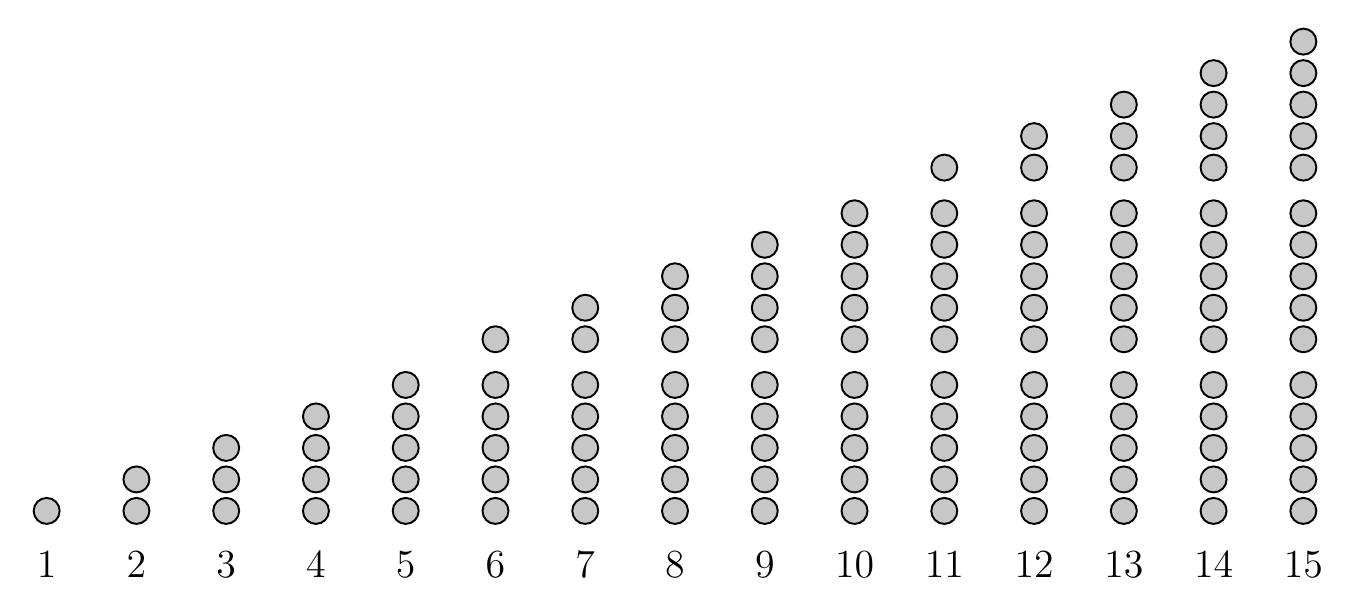
\begin{tikzpicture}
  \foreach \n in {1,...,15}{
    \pgfmathsetmacro{\x}{(\n-1)*1.14}
    \foreach \i in {1,...,\n}{
      \pgfmathsetmacro{\y}{0.25+(\i-1)*0.4+floor((\i-1)/5)*0.18}
      \node[ctr=0.33cm, line width=0.7pt] at (\x,\y) {};
    }
    \node[font=\fontsize{15}{15}\selectfont, anchor=base] at (\x,-0.6) {\n};
  }
\end{tikzpicture}
\end{center}

\vspace{14mm}
\problem{4} Take 1 or 2 each turn, and play a grown-up with 20 counters. You choose who goes first, and you color a star each time you win.

\vspace{8mm}
\begin{center}
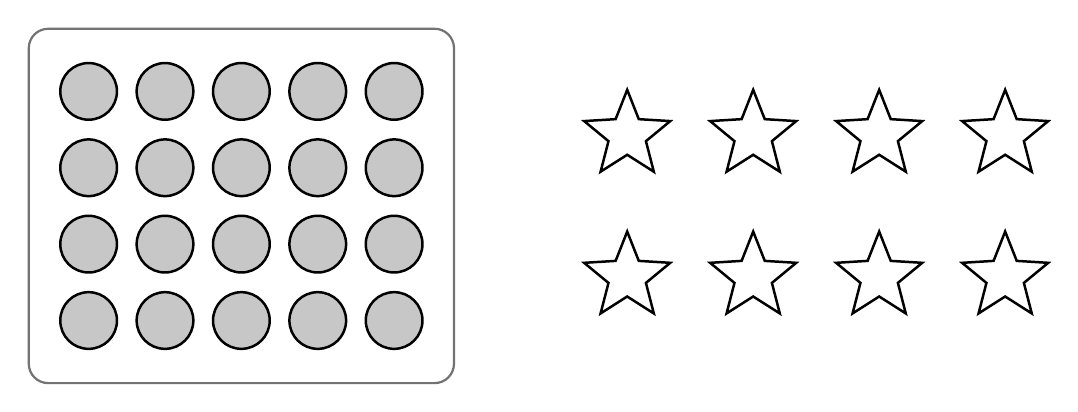
\begin{tikzpicture}
  \pileinbox{20}{0}{0}{5.4}{4.5}{0.97}{ctr=0.72cm}
  \foreach \j in {0,...,3}{
    \node[estar] at ({4.9+\j*1.6},0.9) {};
    \node[estar] at ({4.9+\j*1.6},-0.9) {};
  }
\end{tikzpicture}
\end{center}

% ------------------------------------------------------------------
\newpage
\problem{5} Now take 1, 2, or 3 each turn. Circle 1st or 2nd to show whether you would rather go first or second.

\vspace{10mm}
\begin{center}
\kchoice{3}\hfill\kchoice{4}\hfill\kchoice{5}

\vspace{16mm}
\kchoice{6}\hfill\kchoice{7}\hfill\kchoice{8}
\end{center}

% ------------------------------------------------------------------
\newpage
\problem{6} Now take 1 or 3 each turn, never 2. Color the star under each pile where you can always win if you go first.

\vspace{8mm}
\begin{center}
\kstar{1}\hfill\kstar{2}\hfill\kstar{3}

\vspace{7mm}
\kstar{4}\hfill\kstar{5}\hfill\kstar{6}

\vspace{7mm}
\kstar{7}\hfill\kstar{8}\hfill\kstar{9}
\end{center}

% ------------------------------------------------------------------
\newpage
\problem{7} Take 1 or 2 counters from just one row each turn. Circle whether you would rather go 1st or 2nd, and tell how you win.

\newcommand{\trp}[2]{\tworowpic{#1}{#2}{6.6}{3.0}{1.05}{1.25}{ctr=0.74cm}{%
    \node[choice] at (-1.0,-1.1) {1st};
    \node[choice] at (1.0,-1.1) {2nd};}}
\vspace{12mm}
\begin{center}
\trp{2}{2}\hspace{18mm}\trp{3}{3}

\vspace{14mm}
\trp{2}{3}\hspace{18mm}\trp{4}{4}
\end{center}

\end{document}
